\section{Interfacing the LDR through OpenModelica}
\subsection{Interfacing the LDR}
In this section, we discuss how to carry out the experiments of the
previous section from OpenModelica.  We will list the same two experiments,
in the same order.  The Shield has to be attached to the \arduino\ board
before doing these experiments and the \arduino\ needs to be connected to the computer 
with a USB cable, as shown in \figref{arduino}.
The reader should go through the instructions given in
\secref{sec:OpenModelica-start} before getting started.

\begin{enumerate}
  \item In the first experiment, we will read the LDR values. The code for this experiment is given in
        \OpenModelicaref{OpenModelica:ldr-read} . As explained earlier in \secref{sec:light-OpenModelica}, 
        we begin with importing the two packages: Streams and SerialCommunication followed 
        by setting up the serial port. Then, we read the input coming from analog pin 5 using the 
        following command:
        \lstinputlisting[firstline=16,lastline=16]
        {\LocLDROpenModelicacode/ldr-read.mo} Note that the one leg of the LDR on
        the Shield is connected to analog pin 5 of \arduino\, 
        as given in \figref{fig:ldrconn}. The read value is displayed 
        by the following command: 
        \lstinputlisting[firstline=17,lastline=17]
        {\LocLDROpenModelicacode/ldr-read.mo} where {\tt val} contains
        the LDR values ranging from 0 to 1023. If one does the experiment in a completely dark room, the
        reading will be 0. If on the other hand, a bright light, say for instance the torch
        light from mobile, is shined, the value displayed is close to 1023. One will get
        intermediate values by keeping one's finger on the LDR. While simulating this experiment, the readers must keep their fingertips on the LDR and
        observe the change in values being printed on on the output window of OMEdit, as shown in \figref{om-sim-success}.
        
  \item This experiment is an extension of the previous experiment. Here, depending the resistance of the LDR, we will
        turn the red LED on.  The program for this is available at
        \OpenModelicaref{OpenModelica:ldr-led}.  The value of LDR is read and stored in {\tt
            val}.  In case it is below some threshold (like 300 in \OpenModelicaref{OpenModelica:ldr-led}), 
        it puts a high in pin number 11. From \secref{sec:led-pril}, 
        one can note that this pin is for the red LED. If the LDR value is below 300, 
        the red LED will be on, else, it will be turned off. While running this experiment, the readers 
        must keep their fingertips on the LDR so that the threshold is achieved. Accordingly, 
        they can observe whether the red LED is turned on. 
\end{enumerate}

\subsection{OpenModelica Code}
Unlike other code files, the code/model for running experiments using OpenModelica are 
available inside OpenModelica-Arduino toolbox, as explained in \secref{sec:load-om-toolbox}.
Please refer to \figref{om-examples-toolbox} to know how to locate the experiments. 

\label{sec:ldr-OpenModelica-code}
\addtocontents{OpenModelicad}{\protect\addvspace{\codclr}}

\begin{OpenModelicacode}
  \mcaption{Read and display the LDR values}
  {Read and display the LDR values.  Available at
    Arduino -> SerialCommunication -> Examples -> ldr -> ldr\_read.}
  \label{OpenModelica:ldr-read}
  \lstinputlisting{\LocLDROpenModelicacode/ldr-read.mo}
\end{OpenModelicacode}

\begin{OpenModelicacode}
  \mcaption{Turning the red LED on and off}
  {Turning the red LED on and off.  Available at
    Arduino -> SerialCommunication -> Examples -> ldr -> ldr\_led.}
  \label{OpenModelica:ldr-led}
  \lstinputlisting{\LocLDROpenModelicacode/ldr-led.mo}
\end{OpenModelicacode}





%%%%%%%%OpenMocelica Description Ends 

% \section{Do we need these?  \redcolor{Manas, please answer}}
% \begin{figure}
% \centering
% 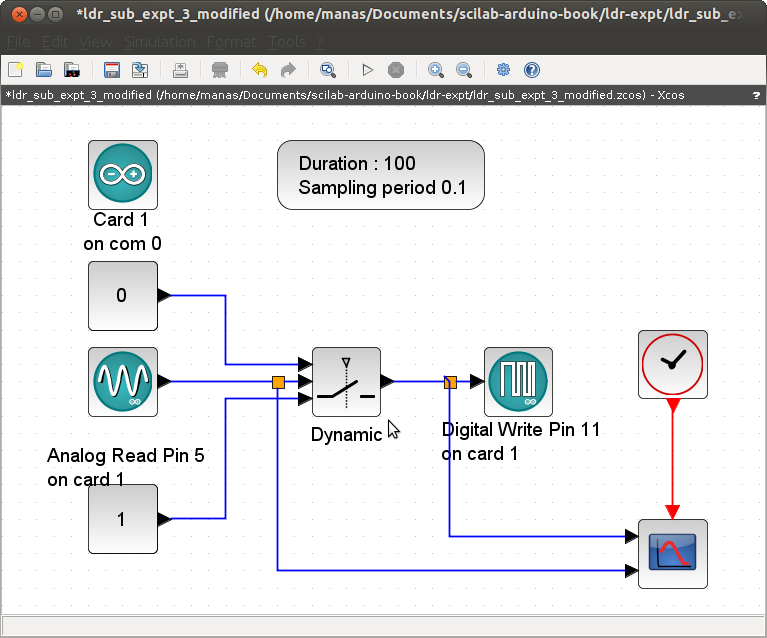
\includegraphics[width=\lgfig]{\LocLDRfig/ldr-led.png}
% \caption{Xcos diagram to change LED state depending on the LDR values}
% \label{fig:ldrxcosled}
% \end{figure}

% \begin{figure}
% \centering
% 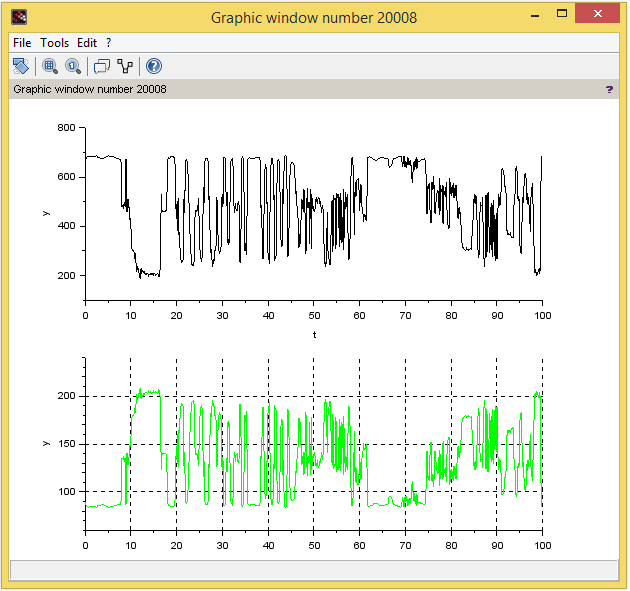
\includegraphics[width=\lgfig]{\LocLDRfig/ldr-led-out.png}
% \caption{LDR output and corresponding LED input}
% \label{fig:ldrledout}
% \end{figure}
%%%%%%%%%%%%%%%%%OpenModelica ends
